\chapter{Related Work}


boilerplate text, boilerplate text, boilerplate text, boilerplate text, boilerplate text, boilerplate text, boilerplate text, boilerplate text, boilerplate text, boilerplate text.


\section{Blockchain Basics}


\subsection{Consensus Algorithms}

Proof-of-Work

Proof-of-Stake


\section{Web Archiving: State of the Art}

\subsection{Web Archiving Standards}


\section{Interactivity}

\subsection{Self-Awareness}

\begin{figure}[h]
    \centering
    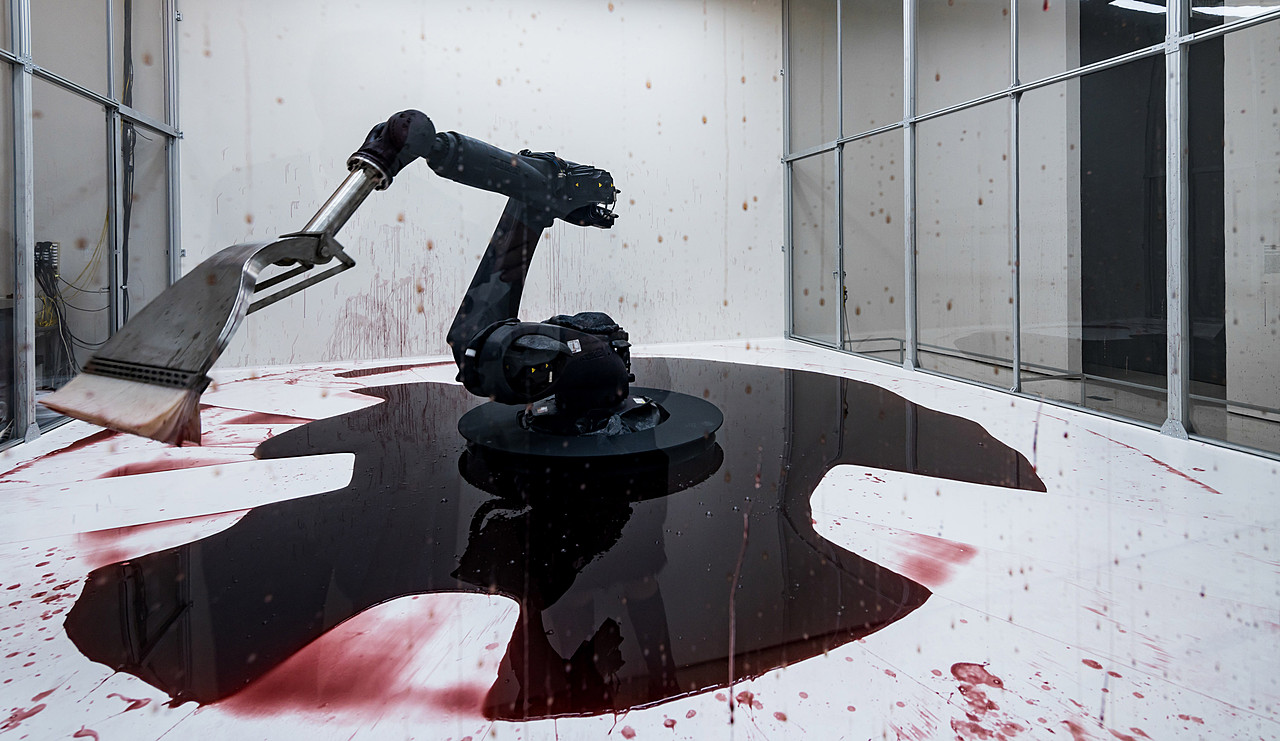
\includegraphics[width=\linewidth]{artwork-robot-cant-help.jpg}
    \caption[Can’t Help Myself by Sun Yuan \& Peng Yu]{Can’t Help Myself by Sun Yuan \& Peng Yu, 2016. Source: https://www.guggenheim.org/artwork/34812}
    \label{fig:robot-canthelp}
\end{figure}


This is a test reference to the work \cref{fig:robot-canthelp}

\subsection{Viewer Interactivity}

\subsection{Network Interactivity}


\section{Decentralisation}
\label{sec:lit_review:decentralisation}


\section{Scalability}

One key aspect to remember is that adding more nodes to a network does not improve network scalability if each node must replicate the exact same computation as every other node, which is the case with most consensus and block validating nodes on a blockchain. Of course such wide replication of computation is still desired, for decentralisation purposes, as discussed in \ref{sec:lit_review:decentralisation}


\subsection{Moore's Law and Data Storage}
